% Options for packages loaded elsewhere
% Options for packages loaded elsewhere
\PassOptionsToPackage{unicode}{hyperref}
\PassOptionsToPackage{hyphens}{url}
\PassOptionsToPackage{dvipsnames,svgnames,x11names}{xcolor}
%
\documentclass[
  letterpaper,
  DIV=11,
  numbers=noendperiod]{scrartcl}
\usepackage{xcolor}
\usepackage[lmargin=0.75in,rmargin=0.75in,tmargin=0.75in,bmargin=0.75in]{geometry}
\usepackage{amsmath,amssymb}
\setcounter{secnumdepth}{-\maxdimen} % remove section numbering
\usepackage{iftex}
\ifPDFTeX
  \usepackage[T1]{fontenc}
  \usepackage[utf8]{inputenc}
  \usepackage{textcomp} % provide euro and other symbols
\else % if luatex or xetex
  \usepackage{unicode-math} % this also loads fontspec
  \defaultfontfeatures{Scale=MatchLowercase}
  \defaultfontfeatures[\rmfamily]{Ligatures=TeX,Scale=1}
\fi
\usepackage{lmodern}
\ifPDFTeX\else
  % xetex/luatex font selection
\fi
% Use upquote if available, for straight quotes in verbatim environments
\IfFileExists{upquote.sty}{\usepackage{upquote}}{}
\IfFileExists{microtype.sty}{% use microtype if available
  \usepackage[]{microtype}
  \UseMicrotypeSet[protrusion]{basicmath} % disable protrusion for tt fonts
}{}
\makeatletter
\@ifundefined{KOMAClassName}{% if non-KOMA class
  \IfFileExists{parskip.sty}{%
    \usepackage{parskip}
  }{% else
    \setlength{\parindent}{0pt}
    \setlength{\parskip}{6pt plus 2pt minus 1pt}}
}{% if KOMA class
  \KOMAoptions{parskip=half}}
\makeatother
% Make \paragraph and \subparagraph free-standing
\makeatletter
\ifx\paragraph\undefined\else
  \let\oldparagraph\paragraph
  \renewcommand{\paragraph}{
    \@ifstar
      \xxxParagraphStar
      \xxxParagraphNoStar
  }
  \newcommand{\xxxParagraphStar}[1]{\oldparagraph*{#1}\mbox{}}
  \newcommand{\xxxParagraphNoStar}[1]{\oldparagraph{#1}\mbox{}}
\fi
\ifx\subparagraph\undefined\else
  \let\oldsubparagraph\subparagraph
  \renewcommand{\subparagraph}{
    \@ifstar
      \xxxSubParagraphStar
      \xxxSubParagraphNoStar
  }
  \newcommand{\xxxSubParagraphStar}[1]{\oldsubparagraph*{#1}\mbox{}}
  \newcommand{\xxxSubParagraphNoStar}[1]{\oldsubparagraph{#1}\mbox{}}
\fi
\makeatother

\usepackage{color}
\usepackage{fancyvrb}
\newcommand{\VerbBar}{|}
\newcommand{\VERB}{\Verb[commandchars=\\\{\}]}
\DefineVerbatimEnvironment{Highlighting}{Verbatim}{commandchars=\\\{\}}
% Add ',fontsize=\small' for more characters per line
\usepackage{framed}
\definecolor{shadecolor}{RGB}{241,243,245}
\newenvironment{Shaded}{\begin{snugshade}}{\end{snugshade}}
\newcommand{\AlertTok}[1]{\textcolor[rgb]{0.68,0.00,0.00}{#1}}
\newcommand{\AnnotationTok}[1]{\textcolor[rgb]{0.37,0.37,0.37}{#1}}
\newcommand{\AttributeTok}[1]{\textcolor[rgb]{0.40,0.45,0.13}{#1}}
\newcommand{\BaseNTok}[1]{\textcolor[rgb]{0.68,0.00,0.00}{#1}}
\newcommand{\BuiltInTok}[1]{\textcolor[rgb]{0.00,0.23,0.31}{#1}}
\newcommand{\CharTok}[1]{\textcolor[rgb]{0.13,0.47,0.30}{#1}}
\newcommand{\CommentTok}[1]{\textcolor[rgb]{0.37,0.37,0.37}{#1}}
\newcommand{\CommentVarTok}[1]{\textcolor[rgb]{0.37,0.37,0.37}{\textit{#1}}}
\newcommand{\ConstantTok}[1]{\textcolor[rgb]{0.56,0.35,0.01}{#1}}
\newcommand{\ControlFlowTok}[1]{\textcolor[rgb]{0.00,0.23,0.31}{\textbf{#1}}}
\newcommand{\DataTypeTok}[1]{\textcolor[rgb]{0.68,0.00,0.00}{#1}}
\newcommand{\DecValTok}[1]{\textcolor[rgb]{0.68,0.00,0.00}{#1}}
\newcommand{\DocumentationTok}[1]{\textcolor[rgb]{0.37,0.37,0.37}{\textit{#1}}}
\newcommand{\ErrorTok}[1]{\textcolor[rgb]{0.68,0.00,0.00}{#1}}
\newcommand{\ExtensionTok}[1]{\textcolor[rgb]{0.00,0.23,0.31}{#1}}
\newcommand{\FloatTok}[1]{\textcolor[rgb]{0.68,0.00,0.00}{#1}}
\newcommand{\FunctionTok}[1]{\textcolor[rgb]{0.28,0.35,0.67}{#1}}
\newcommand{\ImportTok}[1]{\textcolor[rgb]{0.00,0.46,0.62}{#1}}
\newcommand{\InformationTok}[1]{\textcolor[rgb]{0.37,0.37,0.37}{#1}}
\newcommand{\KeywordTok}[1]{\textcolor[rgb]{0.00,0.23,0.31}{\textbf{#1}}}
\newcommand{\NormalTok}[1]{\textcolor[rgb]{0.00,0.23,0.31}{#1}}
\newcommand{\OperatorTok}[1]{\textcolor[rgb]{0.37,0.37,0.37}{#1}}
\newcommand{\OtherTok}[1]{\textcolor[rgb]{0.00,0.23,0.31}{#1}}
\newcommand{\PreprocessorTok}[1]{\textcolor[rgb]{0.68,0.00,0.00}{#1}}
\newcommand{\RegionMarkerTok}[1]{\textcolor[rgb]{0.00,0.23,0.31}{#1}}
\newcommand{\SpecialCharTok}[1]{\textcolor[rgb]{0.37,0.37,0.37}{#1}}
\newcommand{\SpecialStringTok}[1]{\textcolor[rgb]{0.13,0.47,0.30}{#1}}
\newcommand{\StringTok}[1]{\textcolor[rgb]{0.13,0.47,0.30}{#1}}
\newcommand{\VariableTok}[1]{\textcolor[rgb]{0.07,0.07,0.07}{#1}}
\newcommand{\VerbatimStringTok}[1]{\textcolor[rgb]{0.13,0.47,0.30}{#1}}
\newcommand{\WarningTok}[1]{\textcolor[rgb]{0.37,0.37,0.37}{\textit{#1}}}

\usepackage{longtable,booktabs,array}
\newcounter{none} % for unnumbered tables
\usepackage{calc} % for calculating minipage widths
% Correct order of tables after \paragraph or \subparagraph
\usepackage{etoolbox}
\makeatletter
\patchcmd\longtable{\par}{\if@noskipsec\mbox{}\fi\par}{}{}
\makeatother
% Allow footnotes in longtable head/foot
\IfFileExists{footnotehyper.sty}{\usepackage{footnotehyper}}{\usepackage{footnote}}
\makesavenoteenv{longtable}
\usepackage{graphicx}
\makeatletter
\newsavebox\pandoc@box
\newcommand*\pandocbounded[1]{% scales image to fit in text height/width
  \sbox\pandoc@box{#1}%
  \Gscale@div\@tempa{\textheight}{\dimexpr\ht\pandoc@box+\dp\pandoc@box\relax}%
  \Gscale@div\@tempb{\linewidth}{\wd\pandoc@box}%
  \ifdim\@tempb\p@<\@tempa\p@\let\@tempa\@tempb\fi% select the smaller of both
  \ifdim\@tempa\p@<\p@\scalebox{\@tempa}{\usebox\pandoc@box}%
  \else\usebox{\pandoc@box}%
  \fi%
}
% Set default figure placement to htbp
\def\fps@figure{htbp}
\makeatother





\setlength{\emergencystretch}{3em} % prevent overfull lines

\providecommand{\tightlist}{%
  \setlength{\itemsep}{0pt}\setlength{\parskip}{0pt}}



 


\usepackage{multicol}
\KOMAoption{captions}{tableheading}
\makeatletter
\@ifpackageloaded{caption}{}{\usepackage{caption}}
\AtBeginDocument{%
\ifdefined\contentsname
  \renewcommand*\contentsname{Table of contents}
\else
  \newcommand\contentsname{Table of contents}
\fi
\ifdefined\listfigurename
  \renewcommand*\listfigurename{List of Figures}
\else
  \newcommand\listfigurename{List of Figures}
\fi
\ifdefined\listtablename
  \renewcommand*\listtablename{List of Tables}
\else
  \newcommand\listtablename{List of Tables}
\fi
\ifdefined\figurename
  \renewcommand*\figurename{Figure}
\else
  \newcommand\figurename{Figure}
\fi
\ifdefined\tablename
  \renewcommand*\tablename{Table}
\else
  \newcommand\tablename{Table}
\fi
}
\@ifpackageloaded{float}{}{\usepackage{float}}
\floatstyle{ruled}
\@ifundefined{c@chapter}{\newfloat{codelisting}{h}{lop}}{\newfloat{codelisting}{h}{lop}[chapter]}
\floatname{codelisting}{Listing}
\newcommand*\listoflistings{\listof{codelisting}{List of Listings}}
\makeatother
\makeatletter
\makeatother
\makeatletter
\@ifpackageloaded{caption}{}{\usepackage{caption}}
\@ifpackageloaded{subcaption}{}{\usepackage{subcaption}}
\makeatother
\usepackage{bookmark}
\IfFileExists{xurl.sty}{\usepackage{xurl}}{} % add URL line breaks if available
\urlstyle{same}
% fallback for those not using the hyperref driver hyperxmp:
\makeatletter
\@ifundefined{xmpquote}{\newcommand{\xmpquote}[1]{#1}}{}
\makeatother
\hypersetup{
  pdftitle={DATA100 Midterm Version 1 (pink)},
  colorlinks=true,
  linkcolor={blue},
  filecolor={Maroon},
  citecolor={Blue},
  urlcolor={Blue},
  pdfcreator={LaTeX via pandoc}}


\title{DATA100 Midterm Version 1 (pink)\vspace{-0.75cm}}
\author{}
\date{Tuesday, October 6, 2026}
\begin{document}
\maketitle


\textbf{Instructions}: Put your name, WLU id, \textbf{and section} on
the answer sheet (which is separate).

\textbf{Answer all questions on the answer sheet.}

Only the \textbf{answer sheet} will be graded. No answers on this
booklet will be considered. You may use this booklet for scrap paper.

There are 8 pages, with questions printed on the front and back of each
sheet.

\clearpage

\quad

\clearpage

\section{Multiple Choice Questions}\label{multiple-choice-questions}

Each question below is worth one mark. Answer on the \textbf{answer
sheet} provided.

\quad

\begin{enumerate}
\def\labelenumi{\arabic{enumi}.}
\tightlist
\item
  Which of the following plots provides information about which kinds of
  cars have the highest miles per gallon (highway)?
\end{enumerate}

\pandocbounded{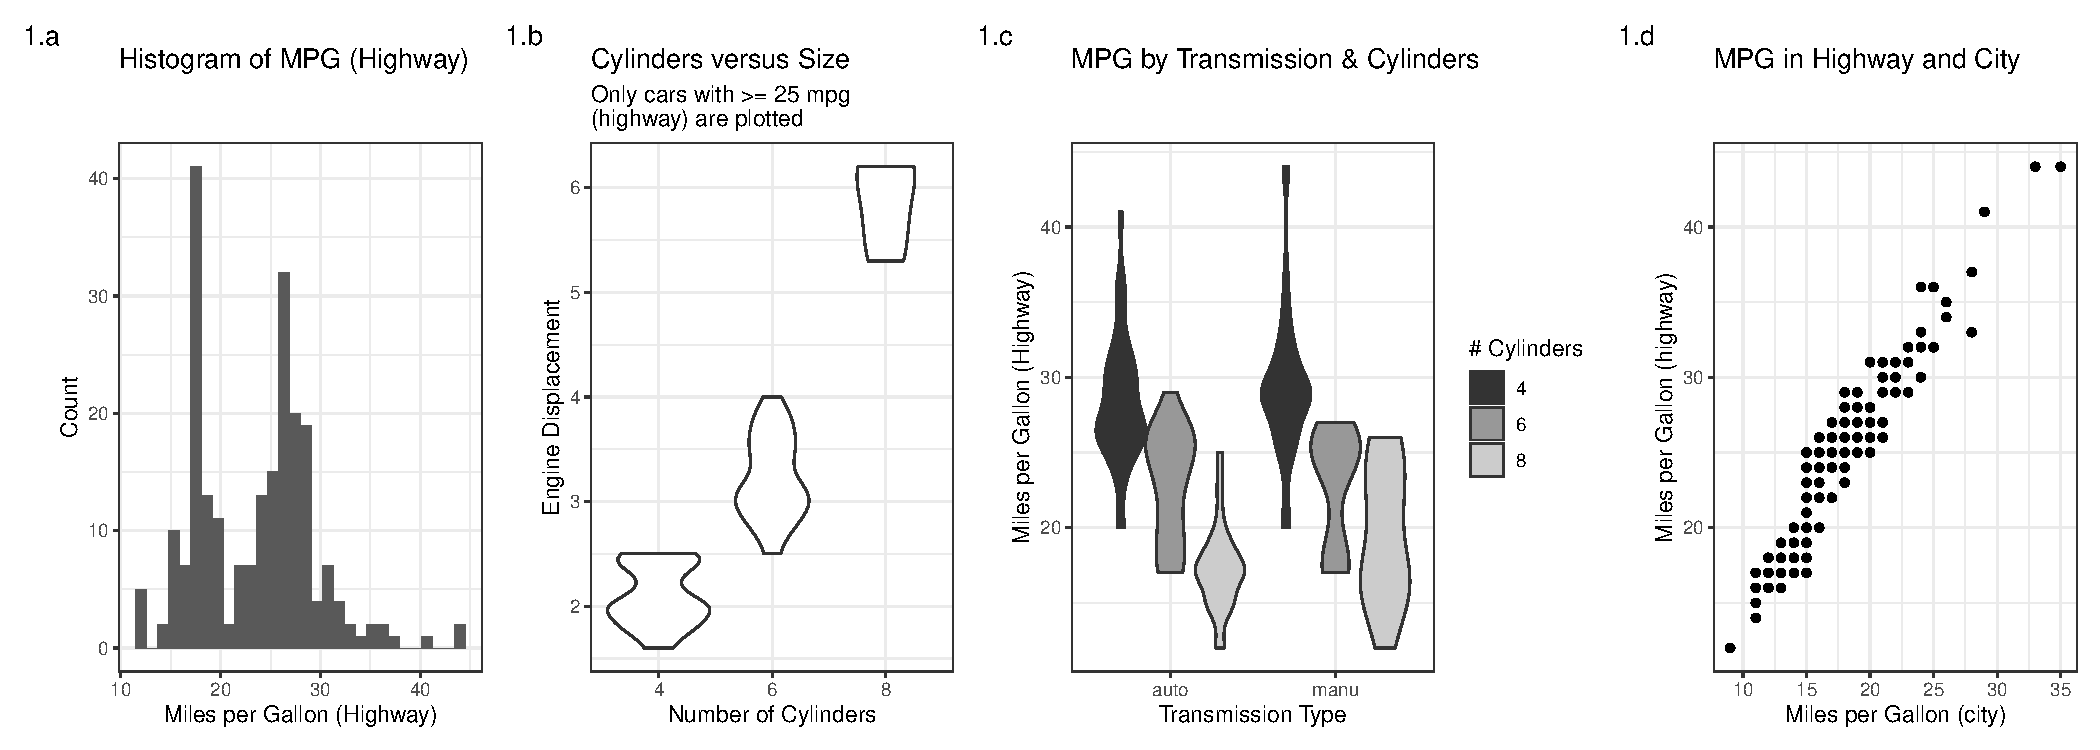
\includegraphics[keepaspectratio]{MT1_F26_files/figure-pdf/unnamed-chunk-2-1.pdf}}

\begin{figure}

\begin{minipage}[t]{0.60\linewidth}

\begin{enumerate}
\def\labelenumi{\arabic{enumi}.}
\setcounter{enumi}{1}
\tightlist
\item
  Which of the following is \textbf{NOT} a valid interpretation of the
  plot on the right?

  \begin{enumerate}
  \def\labelenumii{\alph{enumii}.}
  \tightlist
  \item
    There is an overall decreasing trend when we move from brown to
    green eyes.
  \item
    There were more female subjects than male subjects
  \item
    There were more female subjects with blue and brown eyes than male
    subjects
  \item
    Brown and blue eyes appear to be overall more common than hazel and
    green
  \end{enumerate}
\end{enumerate}

\end{minipage}%
%
\begin{minipage}[t]{0.05\linewidth}

\quad

\end{minipage}%
%
\begin{minipage}[t]{0.35\linewidth}

\pandocbounded{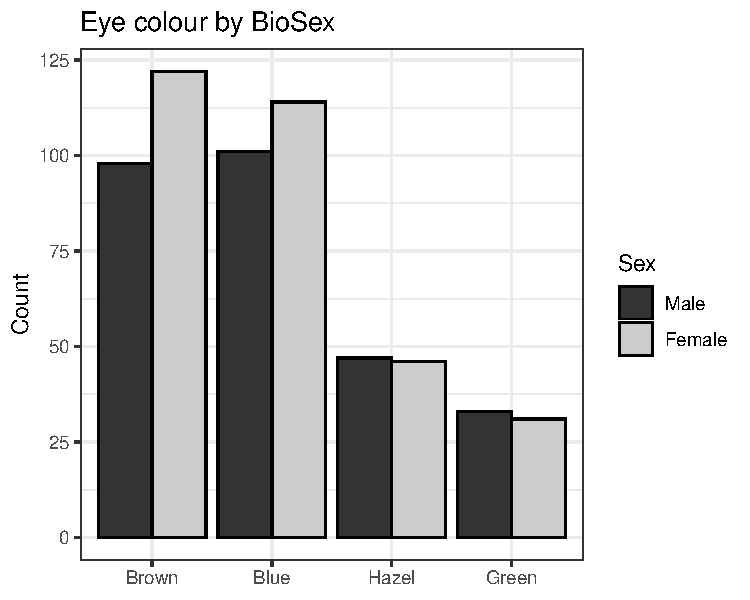
\includegraphics[keepaspectratio]{MT1_F26_files/figure-pdf/unnamed-chunk-3-1.pdf}}

\end{minipage}%

\end{figure}%

\begin{figure}

\begin{minipage}[t]{0.50\linewidth}

\begin{enumerate}
\def\labelenumi{\arabic{enumi}.}
\setcounter{enumi}{2}
\tightlist
\item
  Consider the data on the right. Which of the following plots would
  provide meaningful information?

  \begin{enumerate}
  \def\labelenumii{\alph{enumii}.}
  \tightlist
  \item
    A bar plot of ID versus Name
  \item
    A scatterplot of height versus grade
  \item
    A bar plot of height versus grade
  \item
    A boxplot plot of grade versus year
  \end{enumerate}
\end{enumerate}

\end{minipage}%
%
\begin{minipage}[t]{0.50\linewidth}

{\def\LTcaptype{none} % do not increment counter
\begin{longtable}[]{@{}rlrrr@{}}
\toprule\noalign{}
id & name & height & year & grade \\
\midrule\noalign{}
\endhead
\bottomrule\noalign{}
\endlastfoot
1 & Bonk & 1.2 & 1 & 56 \\
2 & Lilah & 0.4 & NA & NA \\
3 & June & 1.4 & 3 & 88 \\
4 & Judy & 1.6 & 2 & 75 \\
5 & Julie & 1.7 & 1 & 72 \\
6 & Jodie & 1.9 & 1 & 83 \\
7 & Jill & 1.4 & 2 & 81 \\
\end{longtable}
}

\end{minipage}%

\end{figure}%

\begin{enumerate}
\def\labelenumi{\arabic{enumi}.}
\setcounter{enumi}{3}
\tightlist
\item
  In \texttt{ggplot2}, what is the best description of a \texttt{geom}?

  \begin{enumerate}
  \def\labelenumii{\alph{enumii}.}
  \tightlist
  \item
    Declaring the way a data set will be used, e.g.~by assigning columns
    to a dataframe.
  \item
    The way data are assigned to elements of a plot, e.g.~assigning
    \texttt{mpg} to the y axis or assigning \texttt{cyl} to the colour
    scheme.
  \item
    The way elements of a plot are actually drawn, e.g.~by declaring
    that a violin plot will be used.
  \item
    The way additional plot elements, such as arrows or text, are added
    tp the plot.
  \end{enumerate}
\end{enumerate}

\begin{enumerate}
\def\labelenumi{\arabic{enumi}.}
\setcounter{enumi}{4}
\tightlist
\item
  Consider a data set which records the number of cents in each person's
  bank account, where each bank account can only have a whole number of
  cents (no decimals). What type of variable is this?

  \begin{enumerate}
  \def\labelenumii{\alph{enumii}.}
  \tightlist
  \item
    Qualitative - Categorical
  \item
    Qualitative - Ordinal
  \item
    Quantitative - Continuous
  \item
    Quantitative - Discrete
  \end{enumerate}
\end{enumerate}

\begin{enumerate}
\def\labelenumi{\arabic{enumi}.}
\setcounter{enumi}{5}
\tightlist
\item
  Consider the data from Question 5; the number of cents in a person's
  bank account. Which of the following visualization provides the most
  useful information?
\end{enumerate}

\pandocbounded{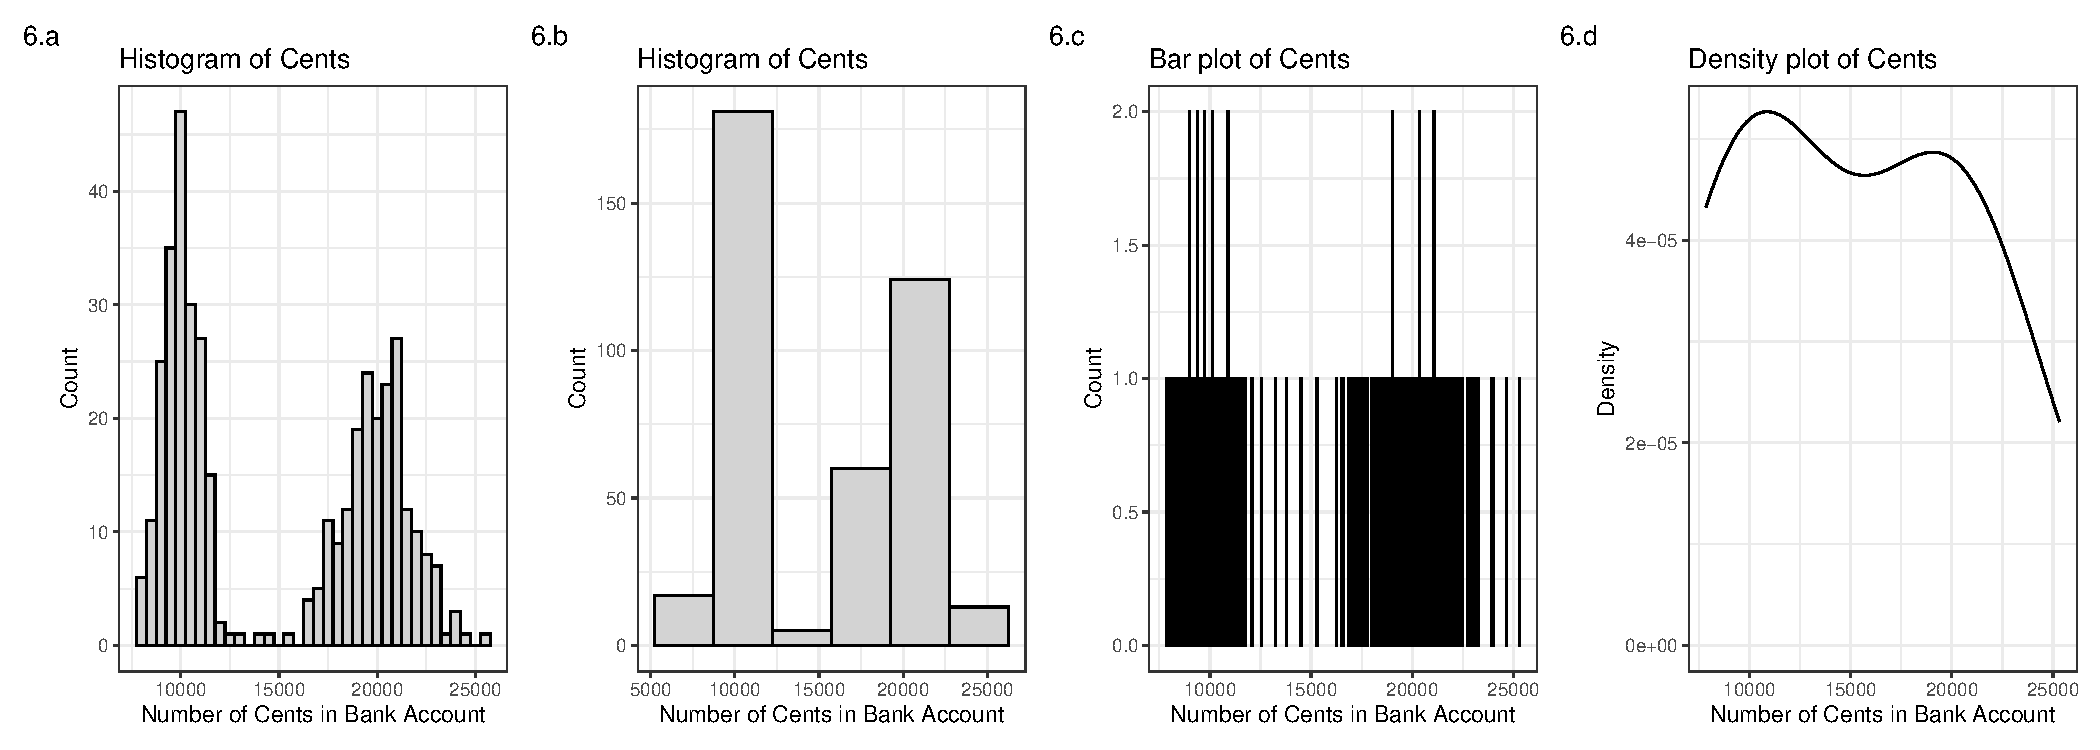
\includegraphics[keepaspectratio]{MT1_F26_files/figure-pdf/unnamed-chunk-5-1.pdf}}

\quad

\begin{figure}

\begin{minipage}[t]{0.52\linewidth}
Consider the plot on the right for the next question. Note that the name
of the data set is \texttt{mpg}, with columns \texttt{class} for the
type of car (sedan, SUV, truck, etc.), \texttt{displ} for the size of
the engine (displacement) in cubic feet, \texttt{hwy} for highway fuel
efficiency in miles per gallon, and \texttt{cyl} for number of cylinders
in the engine.\end{minipage}%
%
\begin{minipage}[t]{0.05\linewidth}

\quad

\end{minipage}%
%
\begin{minipage}[t]{0.43\linewidth}

\pandocbounded{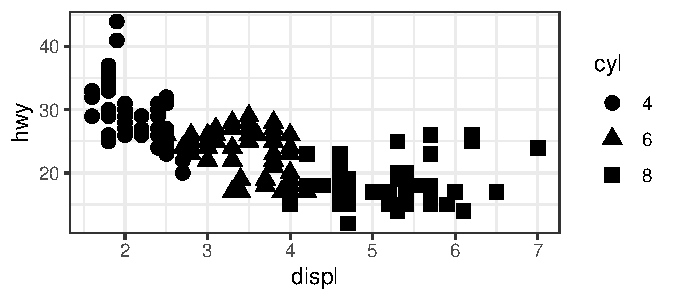
\includegraphics[keepaspectratio]{MT1_F26_files/figure-pdf/unnamed-chunk-6-1.pdf}}

\end{minipage}%

\end{figure}%

\begin{enumerate}
\def\labelenumi{\arabic{enumi}.}
\setcounter{enumi}{6}
\tightlist
\item
  Which code produced the figure above?

  \begin{enumerate}
  \def\labelenumii{\alph{enumii}.}
  \tightlist
  \item
    \texttt{ggplot(mpg)\ +\ aes(x\ =\ displ,\ y\ =\ hwy,\ shape\ =\ cyl)\ +\ geom\_point()}
  \item
    \texttt{ggplot(mpg)\ +\ aes(x\ =\ hwy,\ y\ =\ displ,\ colour\ =\ cyl)\ +\ geom\_point()}
  \item
    \texttt{ggplot(mpg)\ +\ aes(x\ =\ displ,\ y\ =\ hwy,\ colour\ =\ cyl)\ +\ geom\_scatterplot()}
  \item
    \texttt{ggplot(mpg)\ +\ geom\_scatterplot(x\ =\ hwy,\ y\ =\ displ,\ shape\ =\ cyl)}
  \end{enumerate}
\item
  Consider the following code. Which figure would it produce?
\end{enumerate}

\begin{Shaded}
\begin{Highlighting}[]
\FunctionTok{ggplot}\NormalTok{(penguins) }\SpecialCharTok{+}
    \FunctionTok{aes}\NormalTok{(}\AttributeTok{x =}\NormalTok{ species, }\AttributeTok{fill =}\NormalTok{ species) }\SpecialCharTok{+}
    \FunctionTok{geom\_bar}\NormalTok{() }\SpecialCharTok{+}
    \FunctionTok{facet\_wrap}\NormalTok{(}\SpecialCharTok{\textasciitilde{}}\NormalTok{ island) }\SpecialCharTok{+}
    \FunctionTok{coord\_flip}\NormalTok{() }\SpecialCharTok{+}
    \FunctionTok{labs}\NormalTok{(}
        \AttributeTok{x =} \ConstantTok{NULL}\NormalTok{, }\AttributeTok{y =} \StringTok{"Count"}
\NormalTok{    )}
\end{Highlighting}
\end{Shaded}

\pandocbounded{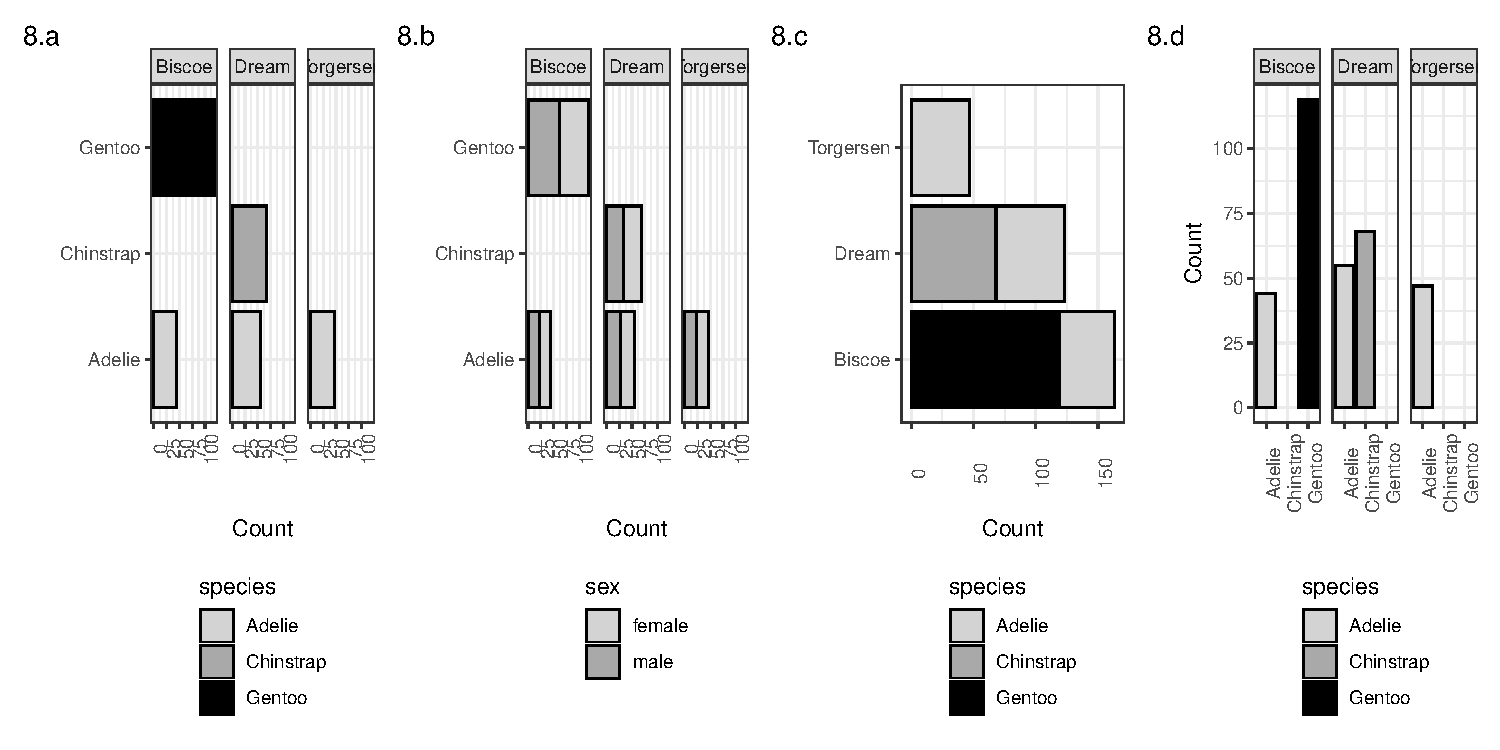
\includegraphics[keepaspectratio]{MT1_F26_files/figure-pdf/unnamed-chunk-8-1.pdf}}

\subsection{Short Answer Questions}\label{short-answer-questions}

\begin{enumerate}
\def\labelenumi{\arabic{enumi}.}
\setcounter{enumi}{15}
\tightlist
\item
  Plot the following data on the axes provided in the answer sheet.
  Choose whichever plot you believe is most appropriate.
\end{enumerate}

\begin{verbatim}
# A tibble: 1 x 3
  grade class     student
  <dbl> <chr>     <chr>  
1     1 chemistry me     
\end{verbatim}




\end{document}
